\documentclass[11pt]{article}

%####### DON'T CHANGE MARGIN SETTINGS ###########
\newcommand{\keywordfont}{\textsc}
\newcommand{\keyword}[1]{%
  \marginpar{\raggedright\small\keywordfont{#1}}}
\reversemarginpar
\usepackage[a4paper, top=2.5cm, bottom=2.5cm, outer=2cm, inner=3.3cm, marginparwidth=72pt, heightrounded]{geometry}
%#################################

\usepackage{amsmath}
\usepackage{amssymb}
\usepackage{hyperref}
\usepackage{graphicx}
\usepackage{microtype}

\begin{document}

\Large
\begin{center}
\textbf{MA3K7 Week $4/5$ Rubric}
\\
Timothy Yap (2161367)
\end{center}
\normalsize



%-----------------------------------------------------------------------------------------------------------

% Matrix game

% You and a friend are playing a game in which you both take turns to write numbers into an n×n
%  grid.

% You can only use the number "0" and your friend can only use the number "1"  in each turn. The game continues until all cells are filled.

% If the final result is a matrix with zero determinant, you win.

% Investigate.



\section{Entry}

We start \keyword{I know} with an empty $n \times n$ grid, I use 0's and my opponent uses 1's to fill up the missing spaces. At the end, we get one of two cases; either a matrix with determinant zero, where I win, or a non-zero determinant, where I lose. 

    We also know the following:
\begin{itemize}
    \item As there are a finite amount of points on this grid and every turn removes one of these points, we know this game will end.
    \item There will always be one winner and one loser (a matrix with a determinant of zero or non-zero)
    \item If $n$ is odd, there will be $\frac{n^2+1}{2}$ 0's and $\frac{n^2-1}{2}$ 1's if I am to start, otherwise there are $\frac{n^2+1}{2}$ 1's and $\frac{n^2-1}{2}$ 0's
    \item If $n$ is even, there will be $\frac{n^2}{2}$ 1's and 0's no matter who goes first
    \item If there is a row or column full of 0's, it will result in a determinant of 0 as we can use said row or column and expansion by cofactors.
    \item This game has perfect information (all players know what moves have occurred) 
    \item Lastly, we know the determinant for a general $2 \times 2$ matrix is 
    $\big(\begin{smallmatrix} 
    a & b\\
    c & d\end{smallmatrix}\big)$
\end{itemize}

Within this game, I want to \keyword{I want} explore the following questions:
\begin{itemize}
    \item Is there a winning strategy? In other words, is there a set of moves that always result in victory?
    \item Who wins if $n$ is odd or even?
    \item Whether who goes first changes who wins?
\end{itemize}

First we \keyword{Introduce} introduce the term '\textit{0-player}' and '\textit{1-player}' where I, 0-player, plays 0's and the 1-player, my friend, plays 1's. We also describe a \textit{turn} when an entry in the matrix is filled. Starting with an empty matrix being turn 0. Lastly, we want to define \textit{strategy} as above; strategy being a set of moves that a player makes, and a \textit{winning strategy} is a strategy that always results in a win.

By specialising, we can immediately see \keyword{Specialise} from below that in the $2 \times 2$ case that the 0-player always wins. No matter if 0-player goes first or second, as there is always a strategy to create a 0 row (some cases are omitted due to symmetry). 
\[
\text{Turn:} \hspace{10pt} 0 \hspace{57pt} 1 \hspace{56pt} 2 \hspace{58pt} 3 \hspace{58pt} 4 \hspace{40pt}
\]
\[ \left( \begin{array}{cc}
\ & \ \\
\ & \
\end{array} \right)
 \rightarrow
%
\left( \begin{array}{cc}
0 & \ \\
\ & \
\end{array} \right)
\rightarrow
%
\left( \begin{array}{cc}
0 & \ \\
1 & \
\end{array} \right)
\rightarrow
%
\left( \begin{array}{cc}
0 & 0 \\
1 & \
\end{array} \right)
\rightarrow
%
\left( \begin{array}{cc}
0 & 0 \\
1 & 1
\end{array} \right)
\]

\[ \left( \begin{array}{cc}
\ & \ \\
\ & \
\end{array} \right)
\rightarrow
%
\left( \begin{array}{cc}
0 & \ \\
\ & \
\end{array} \right)
\rightarrow
%
\left( \begin{array}{cc}
0 & \ \\
\ & 1
\end{array} \right)
\rightarrow
%
\left( \begin{array}{cc}
0 & 0 \\
\ & 1
\end{array} \right)
\rightarrow
%
\left( \begin{array}{cc}
0 & 0 \\
1 & 1
\end{array} \right)
\]

\[ \left( \begin{array}{cc}
\ & \ \\
\ & \
\end{array} \right)
\rightarrow
%
\left( \begin{array}{cc}
1 & \ \\
\ & \
\end{array} \right)
\rightarrow
%
\left( \begin{array}{cc}
1 & \ \\
\ & 0
\end{array} \right)
\rightarrow
%
\left( \begin{array}{cc}
1 & 1 \\
\ & 0
\end{array} \right)
\rightarrow
%
\left( \begin{array}{cc}
1 & 1 \\
0 & 0
\end{array} \right)
\]

Before we begin our attack, \keyword{Assumptions} there are a few assumptions we make. Firstly, we will make it our goal to win. Secondly, we assume 1-player is trying to prevent 0-player from winning and trying to win themselves. Thirdly, all players act rationally on their turn. As this game has perfect information, this implies this game also has Common Knowledge of Rationality. Both 0-player and 1-player decide on their move logically and knowing that it affects their opponent's actions and also know that the other player will make a rational move based on said choice. Now this is a good starting point to begin our attack as we can hopefully generalise our game.



%-----------------------------------------------------------------------------------------------------------



\section{Attack}
Naturally, \keyword{Strategic Specialisation} we now consider $n=3$ . Trying to use the same strategy from the $2 \times 2$ case, we find that there is a counter-strategy to prevent the 0-player from making a 0 row. \keyword{I know} Its common knowledge that Tic-Tac-Toe is a solved game that can always result in a tie. Why bring this up? Because it is analogous to our strategy of trying to create a 0 row. \keyword{Stuck} So we must try and find a different strategy. 

We try \keyword{Try} in Python  to find all possible cases for potential games and come up with 126 different possible games. This comes from 0-player having 5 turns, thus putting 5 0's into our matrix and with 9 choices to place, we get $\binom{9}{5} = 126$ options. After removing any game with a 0 row or column we get 45 different games and only looking at games with a 0 determinant, we have 9 possible games. By symmetry, we get 3 different types of final games as shown below;

\[ 
\left( \begin{array}{ccc}
0 & 1 & 0 \\
1 & 0 & 1 \\
0 & 1 & 0 \\
\end{array} \right)
\hspace{50pt}
%
\left( \begin{array}{ccc}
1 & 0 & 1 \\
0 & 1 & 0 \\
0 & 1 & 0 \\
\end{array} \right)
\hspace{50pt}
%
\left( \begin{array}{ccc}
1 & 1 & 0 \\
0 & 0 & 1 \\
0 & 0 & 1 \\
\end{array} \right)
\]

We are still stuck \keyword{Stuck} as we have yet to find a strategy that the 0-player can use to force a win. However trying to expand by cofactors we notice that  \keyword{AHA} we return to one of the winning cases in the $2 \times 2$ case. 

\begin{figure}[h] % h means put the figure "here"
   \centering
   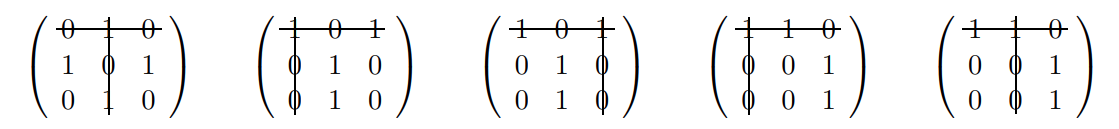
\includegraphics[width=6.2in]{cofactors.png}
   \label{myfig}
\end{figure}

Trying by hand \keyword{Try} we find a winning strategy for when the 0-player starts. We start by putting an 0 in one corner. Depending on where the 1-player plays, we put another 0 next to our initial move so that it forces a 1 to be played to stop us from making a 0-row (shown below). 
\[
\text{Turn:} \hspace{20pt} 0 \hspace{75pt} 1 \hspace{72pt} 2 \hspace{75pt} 3 \hspace{72pt} 4 \hspace{50pt}
\]
\[ \left( \begin{array}{ccc}
\ & \ & \ \\
\ & \ & \ \\
\ & \ & \ \\
\end{array} \right)
\rightarrow
%
\left( \begin{array}{ccc}
0 & \ & \ \\
\ & \ & \ \\
\ & \ & \ \\
\end{array} \right)
\rightarrow
%
\left( \begin{array}{ccc}
0 & \ & 1 \\
\ & \ & \ \\
\ & \ & \ \\
\end{array} \right)
\rightarrow
%
\left( \begin{array}{ccc}
0 & \ & 1 \\
0 & \ & \ \\
\ & \ & \ \\
\end{array} \right)
\rightarrow
%
\left( \begin{array}{c|cc}
0 & \ & 1 \\
0 & \ & \ \\
\hline
1 & \ & \ \\
\end{array} \right)
\]

\[ \left( \begin{array}{ccc}
0 & \ & \ \\
\ & \ & 1 \\
\ & \ & \ \\
\end{array} \right)
\rightarrow
%
\left( \begin{array}{ccc}
0 & 0 & \ \\
\ & \ & 1 \\
\ & \ & \ \\
\end{array} \right)
\rightarrow
%
\left( \begin{array}{cc|c}
0 & 0 & 1 \\
\hline
\ & \ & 1 \\
\ & \ & \ \\
\end{array} \right)
\hspace{5pt} \text{or} \hspace{5pt}
%
\left( \begin{array}{ccc}
0 & \ & \ \\
\ & \ & \ \\
\ & \ & 1 \\
\end{array} \right)
\rightarrow
%
\left( \begin{array}{ccc}
0 & 0 & \ \\
\ & \ & \ \\
\ & \ & 1 \\
\end{array} \right)
\rightarrow
%
\left( \begin{array}{cc|c}
0 & 0 & 1 \\
\hline
\ & \ & \ \\
\ & \ & 1 \\
\end{array} \right)
\]
\[
\text{Turn: } 2 \hspace{75pt} 3 \hspace{72pt} 4 \hspace{90pt} 2 \hspace{72pt} 3 \hspace{73pt} 4 
\]
\[ \left( \begin{array}{ccc}
0 & \ & \ \\
\ & \ & \ \\
\ & 1 & \ \\
\end{array} \right)
\rightarrow
%
\left( \begin{array}{ccc}
0 & 0 & \ \\
\ & \ & \ \\
\ & 1 & \ \\
\end{array} \right)
\rightarrow
%
\left( \begin{array}{cc|c}
0 & 0 & 1 \\
\hline
\ & \ & \ \\
\ & 1 & \ \\
\end{array} \right)
\hspace{5pt} \text{or} \hspace{5pt}
%
\left( \begin{array}{ccc}
0 & \ & \ \\
\ & \ & \ \\
1 & \ & \ \\
\end{array} \right)
\rightarrow
%
\left( \begin{array}{ccc}
0 & 0 & \ \\
\ & \ & \ \\
1 & \ & \ \\
\end{array} \right)
\rightarrow
%
\left( \begin{array}{cc|c}
0 & 0 & 1 \\
\hline
\ & \ & \ \\
1 & \ & \ \\
\end{array} \right)
\]

We show turn 0 and 1 for the first potential game but all other games follow from the first turn. We also end on turn 4 as it is 0-players move and we've already shown in Entry that they can win. Thus 0-player wins in the $3 \times 3$ case when they go first. We now will attempt to adapt a strategy for 0-player when they go second. Similarly to above, we found all possible winning games in Python and after working through some examples, we have a winning strategy which leads to our first conjecture:

\textbf{Winning Strategy for $n = 3$} \keyword{Conjecture} \\
\textbf{Step 1 -} Play a 0 in the intersection of an empty row and empty column. \\
\textbf{Step 2 -} Choose the same row or column as our initial 0 that doesn't have a 1 in it.\\
\textbf{Step 3.A -} If 0-player played first, play a 0 adjacent to our initial 0.\\
\textbf{Step 3.B -} If 0-player played second, in row or column chosen in Step 2, place an 0 where it forces the 1-player to put a 1 in a column or row that already has a 1.\\
\textbf{Step 4 -} Following from the $2 \times 2$ case, create a minor matrix with determinant 0.

To justify, \keyword{Justify} there is always an option for the 0-player to play following step 1, as shown below. The other cases follow through rotational symmetry.
\[ \left( \begin{array}{cc|c}
1 & \ & \ \\
\ & \ & \ \\
\hline
\ & \ & 0 \\
\end{array} \right)
\hspace{40pt}
%
\left( \begin{array}{cc|c}
\ & 1 & \ \\
\ & \ & \ \\
\hline
\ & \ & 0 \\
\end{array} \right)
\hspace{40pt}
%
\left( \begin{array}{cc|c}
\ & \ & \ \\
\ & 1 & \ \\
\hline
\ & \ & 0 \\
\end{array} \right)
\hspace{50pt}
%
\]
To justify Step 2, we can always form a situation where the 1-player is forced to prevent a 0-row from being created. This is due to the fact that we place a 0 in the intersection of an empty row and column. So if 1-player plays a 1 in either the row or column, we can place a 0 in the column or row. 
\[ \left( \begin{array}{cc|c}
1 & \ & \ \\
\ & \ & \ \\
\hline
\ & \ & 0 \\
\end{array} \right)
\hspace{10pt} \rightarrow\hspace{10pt}
%
\left( \begin{array}{ccc}
1 & \ & \ \\
\ & \ & 1 \\
\hline
\ & \ & 0 \\
\end{array} \right)
\hspace{10pt} \text{or} \hspace{10pt}
%
\left( \begin{array}{cc|c}
1 & \ & \ \\
\ & \ & \ \\
\ & 1 & 0 \\
\end{array} \right)
\hspace{50pt}
%
\]
The 0-player can play a 0 in one of two positions, as in this row or column one point is already taken up by our initial 0. If we chose a row from Step 2, There will be at least one column with a 1 that intersects said row. We just play a 0 in the other position and this forces a minor matrix that is winnable by following the $2 \times 2$ case.

With two cases having winning strategies for the 0-player, this pattern may generalise.

This leads us to our second conjecture: \keyword{Conjecture} There is always a winning strategy for the 0-player to win when starting first.

Whilst working \keyword{Stuck} on a way to generalise this, I've found it difficult as increasing values of $n$ makes it exponentially more difficult to keep checking for various winning strategies. We are unable to state our conjecture as fact. So pivoting from this, my aim is to \keyword{Try} try a different strategy.  Relating to another module, IB3J3: Mathematical Game Theory, we learned about a copy-cat strategy, that may be applicable. We may try to create some form of linear dependency. We see this in both the $n=2$ and  $n=3$ case that there is always column or row are linearly dependent on the other column or row. Checking \keyword{Check} our possible winnable games in Python, we see that this is the case. There is a pair of columns or rows that are linearly dependent.

In the $4 \times 4$  case, \keyword{Specialise} we can try copying where 1 is played and play in the adjacent column, thus coupling a position with an adjacent position, and if we do this for a pair of columns or row, we hopefully end with a determinant of 0. Trying to achieve something similar to below:
\[
\left( \begin{array}{cccc}
A & A & W & W \\
B & B & X & X \\
C & C & Y & Y \\
D & D & Z & Z \\
\end{array} \right)
\]

Checking \keyword{Check} with Python, we find that there are $2^8 = 256$ different games. With $n$ even, it doesn't matter who goes first in the copycat strategy as the 0-player can always just play a 0 random initially and follow 1-player. If 1 player plays on the pair that the initial 0 is played, the 0-player can just random put a 0 and take this as the new initial 0 in case 1-player plays in this pair. If 1-player goes first, we just copy as usually. If we generalise \keyword{Generalise}, for even $n$, we have $2^{n \times(n/2)}$ cases. For our $n=4$ case, there are 8 different letters above, thus $2^8$. With $n=6$ we have $2^{6 \times 3}=2^{18}=262144$ cases and with $n=8$ we have $2^{8 \times 4}=2^{32}=4294967296$. We can easily check \keyword{Check} with Python for $n=6$ that the strategy works and none of the potential games have a non-zero determinant. As for $n=8$ we check some cases and also come to the conclusion that this strategy works.

Before generalising our strategy for odd $n$, we explain why this is strategy works. As below, we see one potential case for a $4 \times 4$ game. We first notice that there are no 0 rows or columns or duplicate rows. A rational 1-player would try and prevent this from occurring. Next we notice that the sum of the first and second column is the same as the sum of the second-last and last column. This causes a linear dependency between the columns, resulting in a determinant of 0. 

\[
\left( \begin{array}{cccc}
0 & 1 & 1 & 0 \\
0 & 1 & 0 & 1 \\
1 & 0 & 0 & 1 \\
1 & 0 & 1 & 0 \\
\end{array} \right)
\]
By this logic, we don't actually need the rest of the columns to be copied in cases $n > 4$ as 4 columns are enough to create linear dependency. Thus in the case that $n \geq 5$ and is odd, we can just ignore one of the columns, for example the last column. If 1-player plays in said column, 0-player may take the pairs of columns to be $(2, 3)$ and $(4,5)$ and ignore the first column. With all odd cases taken care of we now state this in the following conjecture:

The copycat strategy \keyword{Conjecture} of mirroring our opponents moves within any two pairs of four columns creates linear dependency as the sum the first two columns is equal to the sum of the third and fourth columns. This results in a determinant of 0.

We know that a \keyword{Justification} matrix is linearly dependent if and only if it is has a determinant of 0. Thus, by playing a copycat strategy within just the first four columns, we can force this to be the outcome. This is the case for any $n \geq 4$. As long as the 0-player plays next to any 1 immediately after 1-player's turn, then this will happen. We also note that no matter who goes first, 0-player can always follow the strategy. This has been checked \keyword{Check} for suitable $n$ values on Python and as expected, all show a determinant of 0. Thus we have a generalised strategy for $n\geq 4$ based on creating linear dependencies. 



%-----------------------------------------------------------------------------------------------------------



\section{Review}

Reviewing the \keyword{Check} questions I had wanted to investigate in the Entry phase, I have managed to answer all. We found a winning strategy for the 0-player which does not matter if $n$ is odd or even and also does not change depending on who goes first. Our initial assumptions of a logical player made our strategy much more rigorous as we had to expect that our opponent understands why we make moves the way we do, and can react accordingly. 

Overall, \keyword{Reflect} I am proud that I found strategies for $n=2$ and $n=3$ and a general strategy for $n \geq 4$ and therefore solving this game. 

Looking back, I initially  had the number of 1's and 0's in an $n \times n$ game wrong as I forgot to square. This came up when coding in Python and indexing become a problem. Luckily this was a minor correction. 
However a major issue I had we trying to generalise my initial attempt of a strategy. It works for small cases as I accounted for it but moving to larger values of $n$, it immediately became obvious that it wasn't the correct method. 

Despite this setback, it still managed to give me insight to linear dependencies as printing the winnable cases in Python showed this for the $3 \times 3$ case. In that case, we see that there is always a duplicate column and thus linear dependencies but this had to be adapted to the $4 \times 4$ case a little differently. In fact, even with the $2 \times 2$ case, we stated the formula for the determinant, but realising we needed either one of $a$ or $d$ to be 0 and either one of $c$ or $b$ to be 0 was another key moment. 

Lastly, this being a game, it reminded me to connect to game theory and my related modules. Said module explored combinatorial games and had helped immensely.

Similar to the previous assignment, Python \keyword{Reflect} was vital in computing large amounts of data. Considering the $n=4$ alone had 256 different cases, checking my strategy would have taken exceptionally long. Despite this, Python can only do so much as checking $n=6$ took about a second for my computer to compute but considering $n=8$ has 4294967296 different cases, it would roughly take $\frac{4294967296}{262144} = 16384 = 2^{14}$ times longer, or about 4.5 hours (if it scales linearly). 

This relates to optimisation as we are currently taking a brute-force approach and checking redundant cases. For example, a rational player wouldn't let duplicate rows form or rows or columns of 0's to form either. Removing this would significantly reduce computation but is a little beyond the scope of this paper and relates more to MA398: Matrix Analysis \& Algorithms and other subjects like computer science and discrete mathematics.
 
There are a few ways to \keyword{Extend} explore this further:
\begin{itemize}
    \item Multiple matrices where they get multiplied before finding the determinant
    \begin{itemize}
        \item This could mean $n \times n$ matrix multiplied by another $n \times n$ matrix but knowing det(AB) = det(A) $ \times $ det(B), 0-player still wins.
        \item Other versions may include $n \times m$ multiplied by $m \times n$ to give a final result of the determinant of an $n \times n$ matrix.
    \end{itemize}
    \item Players may be allowed to play multiple turns before swapping over
    \item What other strategies may work?
\end{itemize}

Taking a small example of having two \keyword{Specialise} games, one $n \times m$ game multiplied by $m \times n$ game, we see the following:

\[
A = (a \hspace{5pt} b), \hspace{20pt} B = \binom{c}{d}, \hspace{20pt} AB = (ac + bd), \hspace{20pt} BA = \binom{ac \hspace{5pt} ad}{bc \hspace{5pt} bd}
\]
Which again leads to 0-player winning as in either cases, 0-player can play one 0 in A and one 0 in B, thus det(AB) $= 0 + 0 = 0$ or det(BA) $= abcd - abcd = 0$. Even going beyond to a $2 \times 3$ and a $3 \times 2$ game, it was difficult to use the copycat strategy as is and will require some tweaking before it is usable. Checking \keyword{Check} a few different games with Python returns in determinants of 1, $-1$ and 0. Exploring further may result in unsolvable games or ones that may even require super computers, in a similar vein that computers was initially used to help prove the Four Colour Theorem.


\section*{Supplementary material}
The code for this assignment can be found on my GitHub page:  \url{https://github.com/LazyTim/MA3K7/blob/main/MA3K7%20-%20Assignment%202.ipynb}.

\end{document}
